\section{Evaluation}
\label{slab:sec:eval}





\begin{figure*}[!t]
\centering
% NOTE (dissertation): re-laid out from the paper's 1x4 strip to a 2x2 grid.
\begin{minipage}[t]{.48\linewidth}\centering
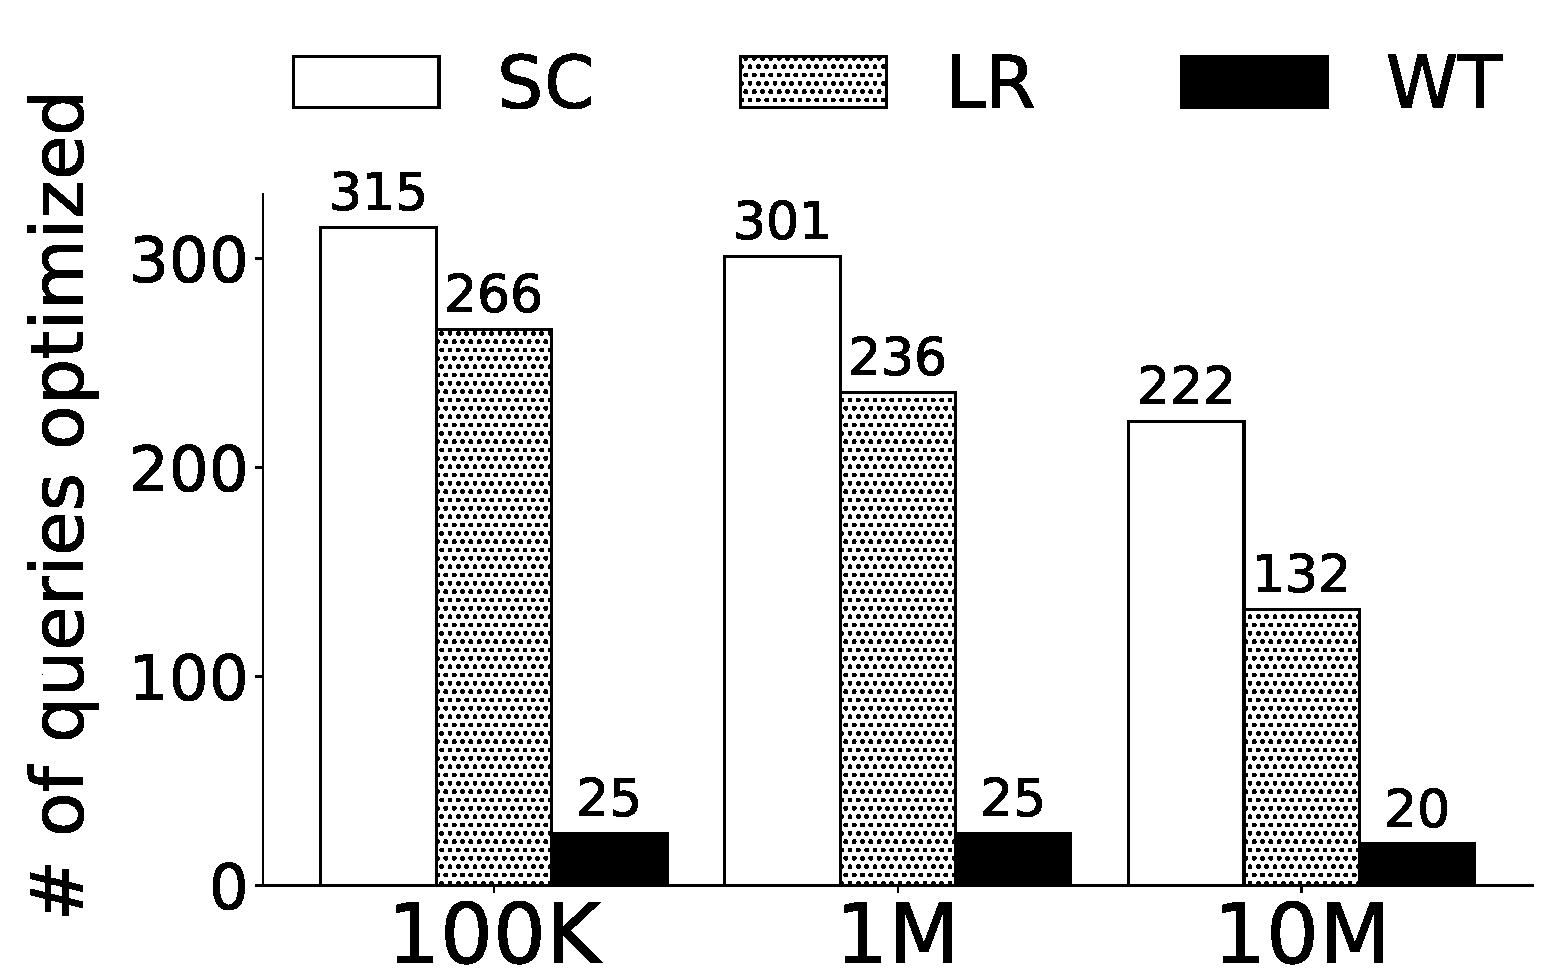
\includegraphics[width=\linewidth]{chapters/slabcity/figs/coverage_LeetCode_time.pdf}
\caption*{\small (a) Coverage (\# of queries).}
\label{slab:fig:leetcode-coverage}
\end{minipage}\hfill
\begin{minipage}[t]{.48\linewidth}\centering
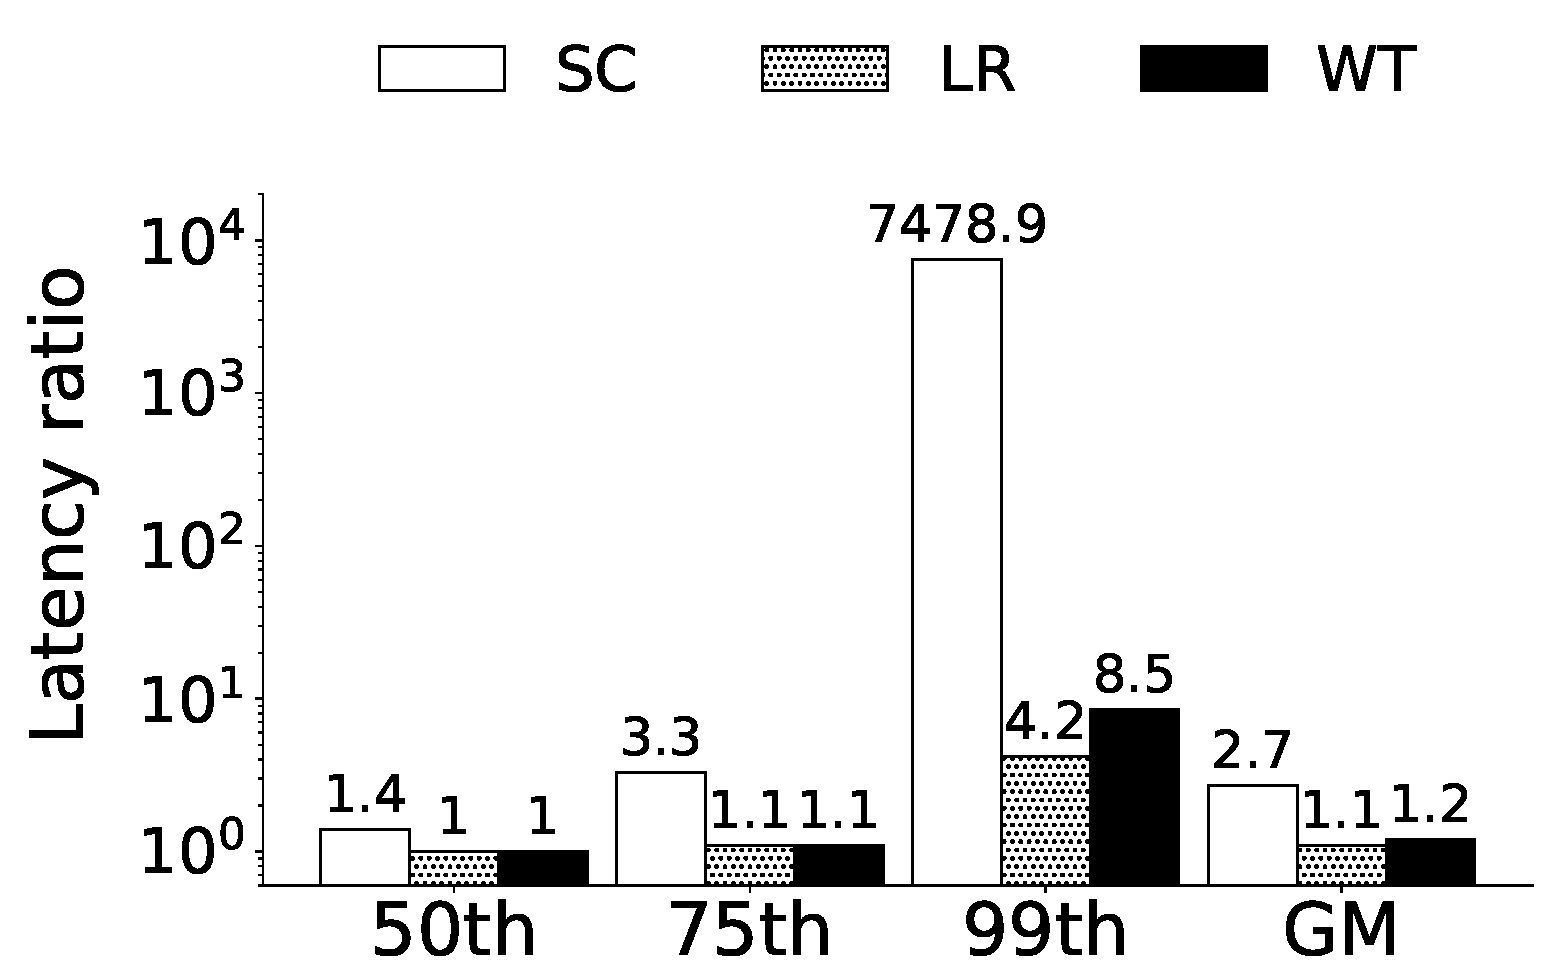
\includegraphics[width=\linewidth]{chapters/slabcity/figs/time_LeetCode_100K.pdf}
\end{minipage}\\[8pt]
\begin{minipage}[t]{.48\linewidth}\centering
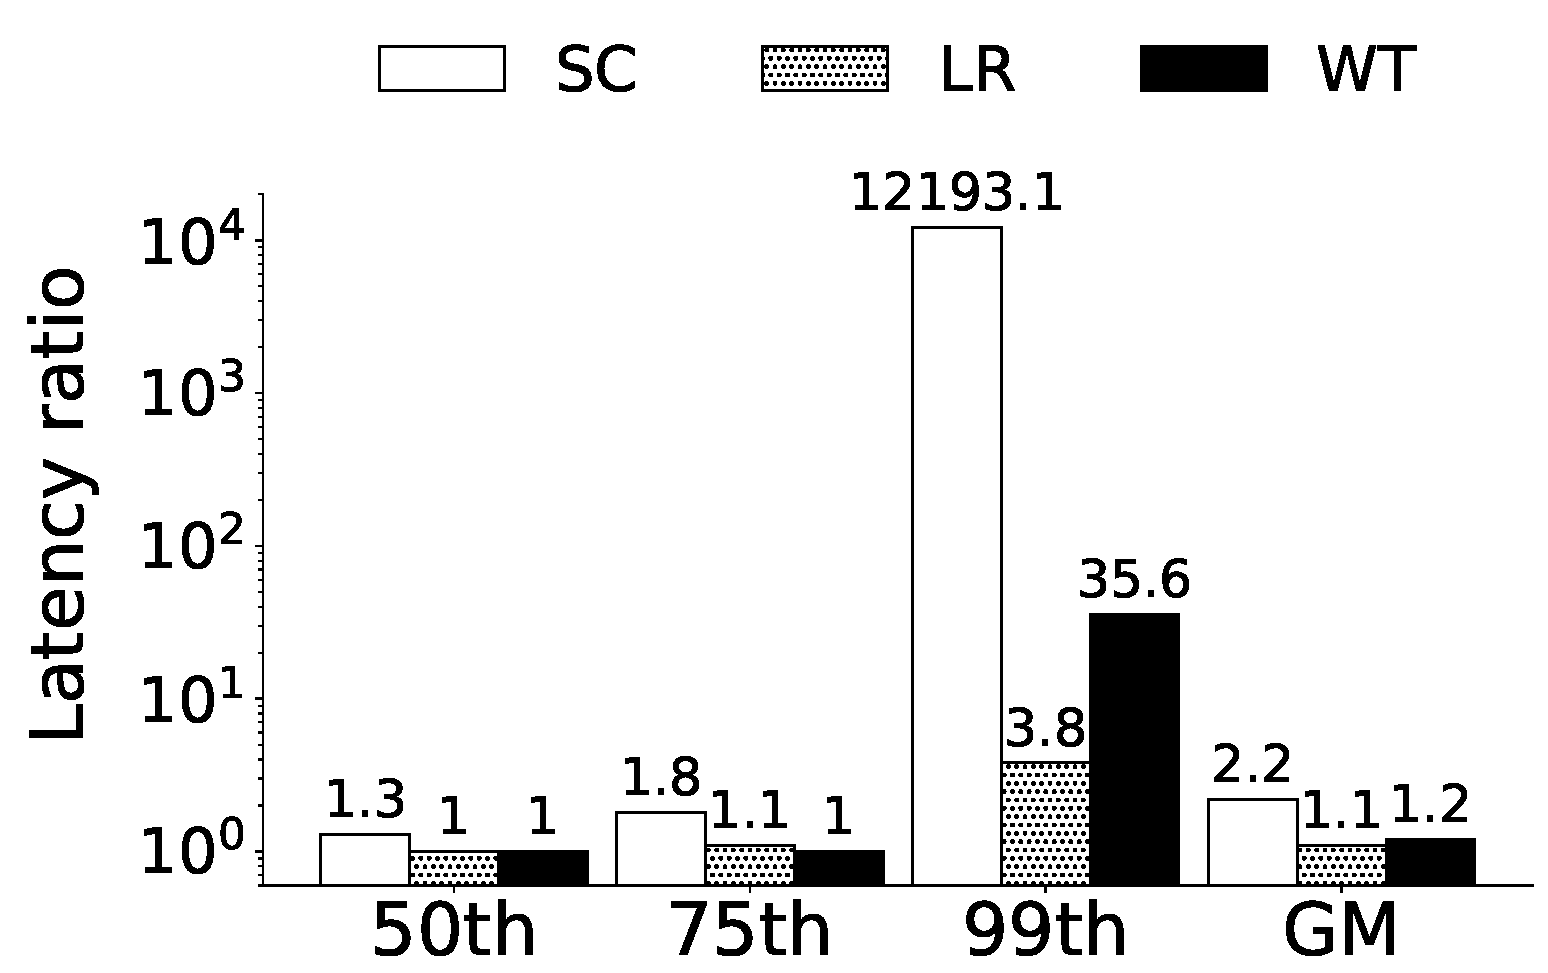
\includegraphics[width=\linewidth]{chapters/slabcity/figs/time_LeetCode_1M.pdf}
\end{minipage}\hfill
\begin{minipage}[t]{.48\linewidth}\centering
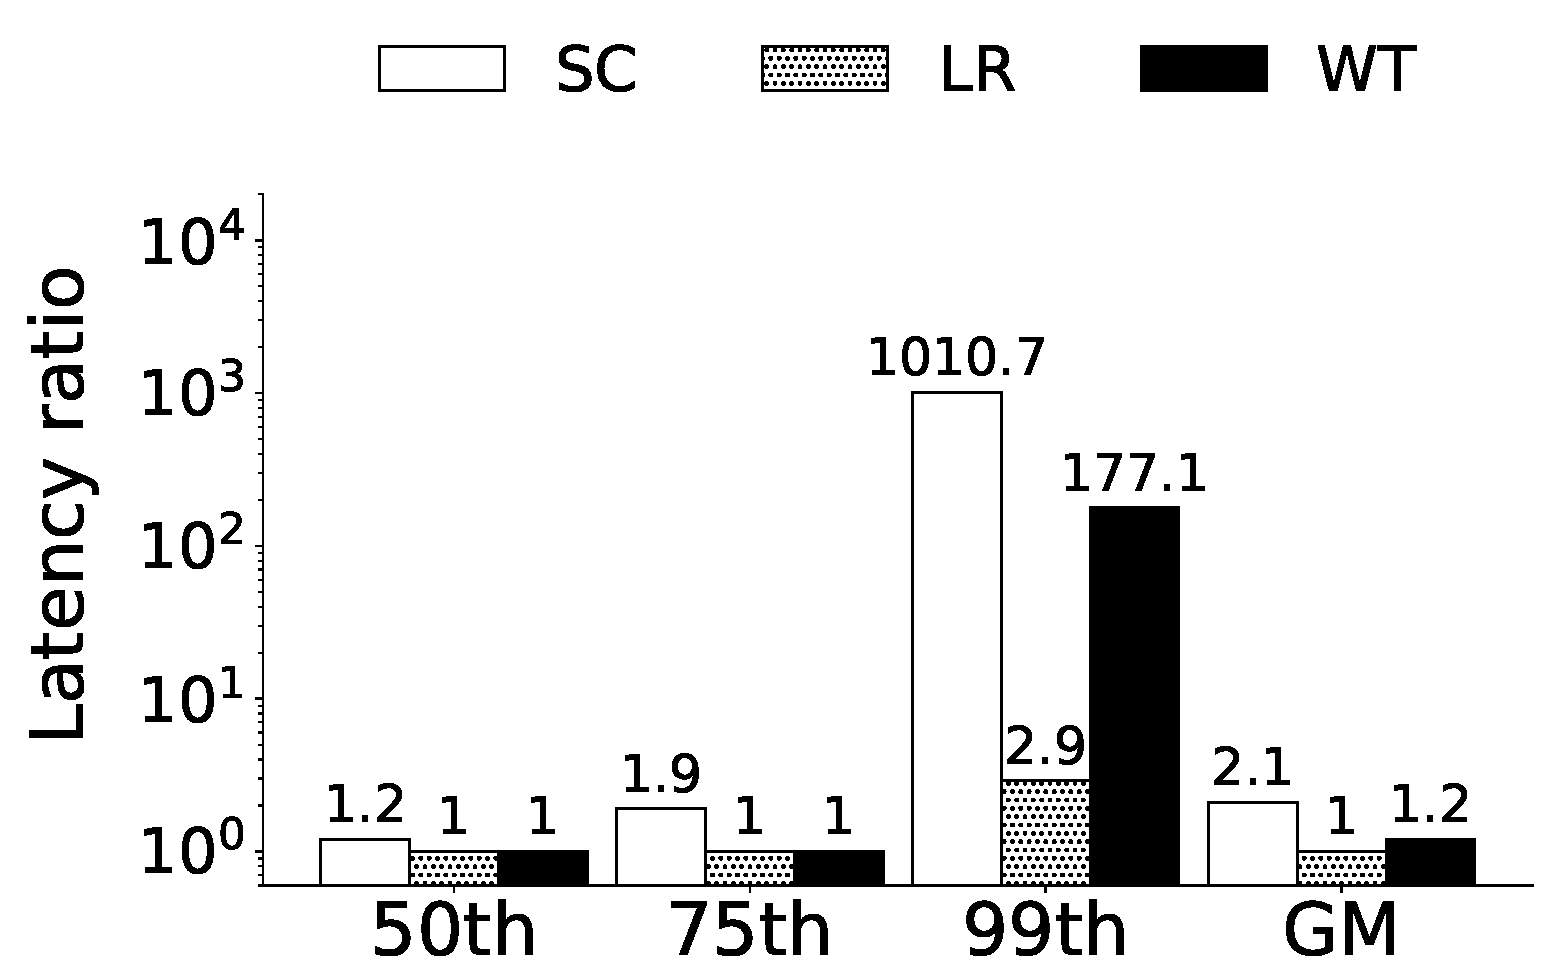
\includegraphics[width=\linewidth]{chapters/slabcity/figs/time_LeetCode_10M.pdf}
\end{minipage}
\caption*{\small (b) Latency reduction: top right is on 100K, bottom left is on 1M, and bottom right is on 10M. ``GM'' means geometric mean.}
\label{slab:fig:leetcode-reduction-latency}
\caption{\barzanrev{LeetCode results across all data sizes with uniform distribution.}}
\label{slab:fig:leetcode-results}
\end{figure*}




\begin{figure*}[!t]
\centering
% NOTE (dissertation): re-laid out from the paper's 1x4 strip to a 2x2 grid.
\begin{minipage}[t]{.48\linewidth}\centering
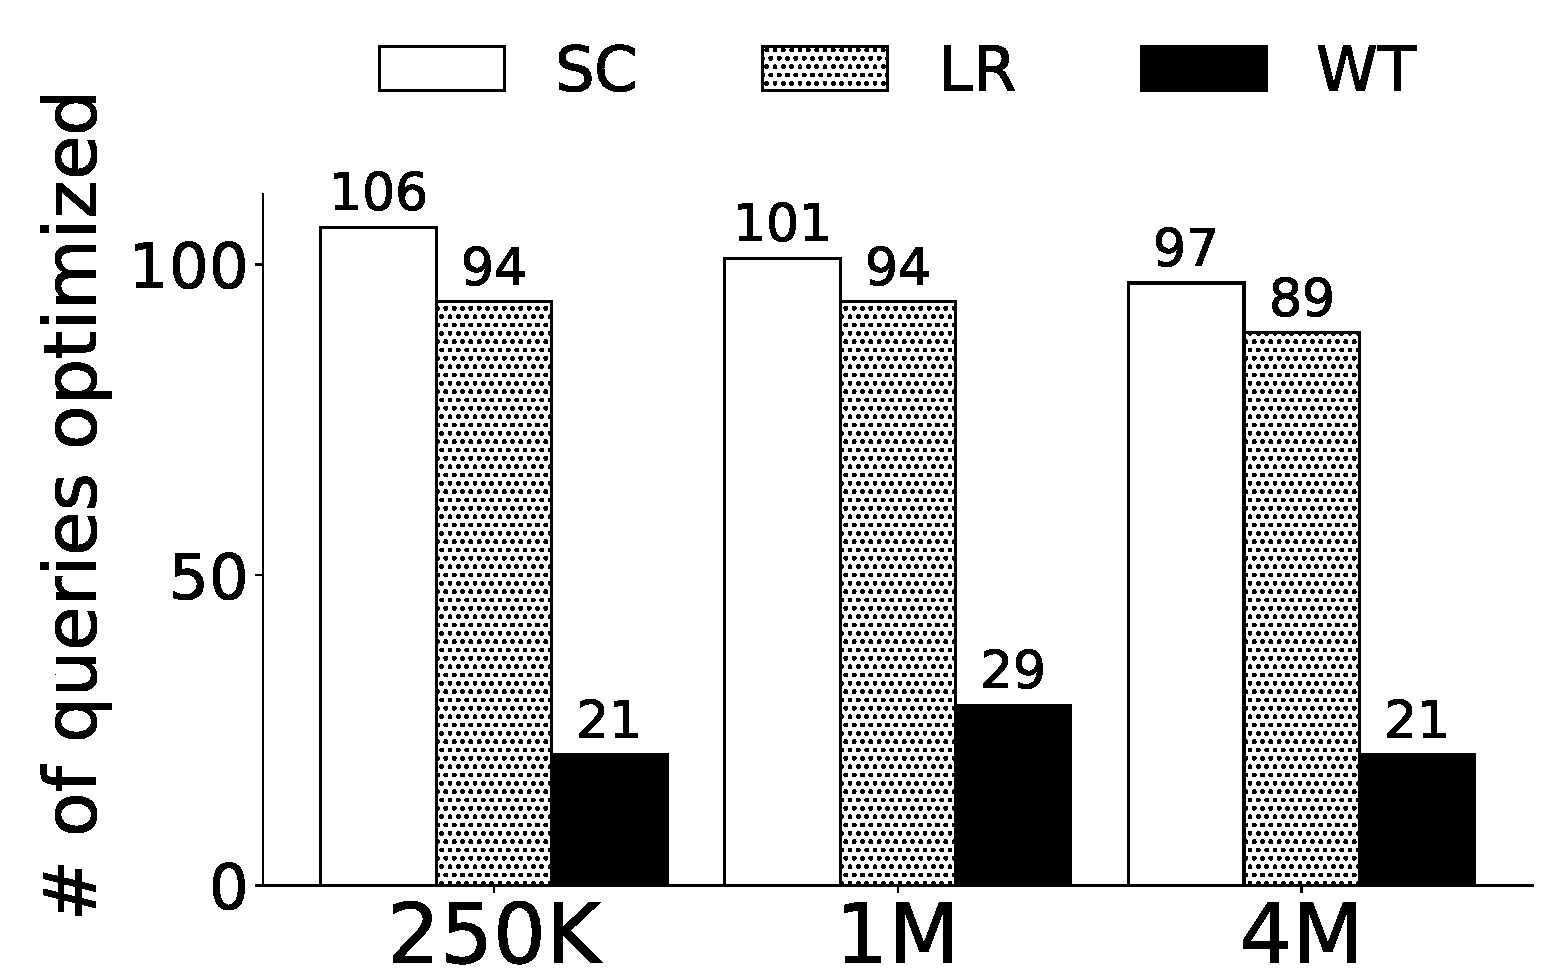
\includegraphics[width=\linewidth]{chapters/slabcity/figs/coverage_Calcite_time.pdf}
\caption*{\small (a) Coverage (\# of queries).}
\label{slab:fig:calcite-coverage}
\end{minipage}\hfill
\begin{minipage}[t]{.48\linewidth}\centering
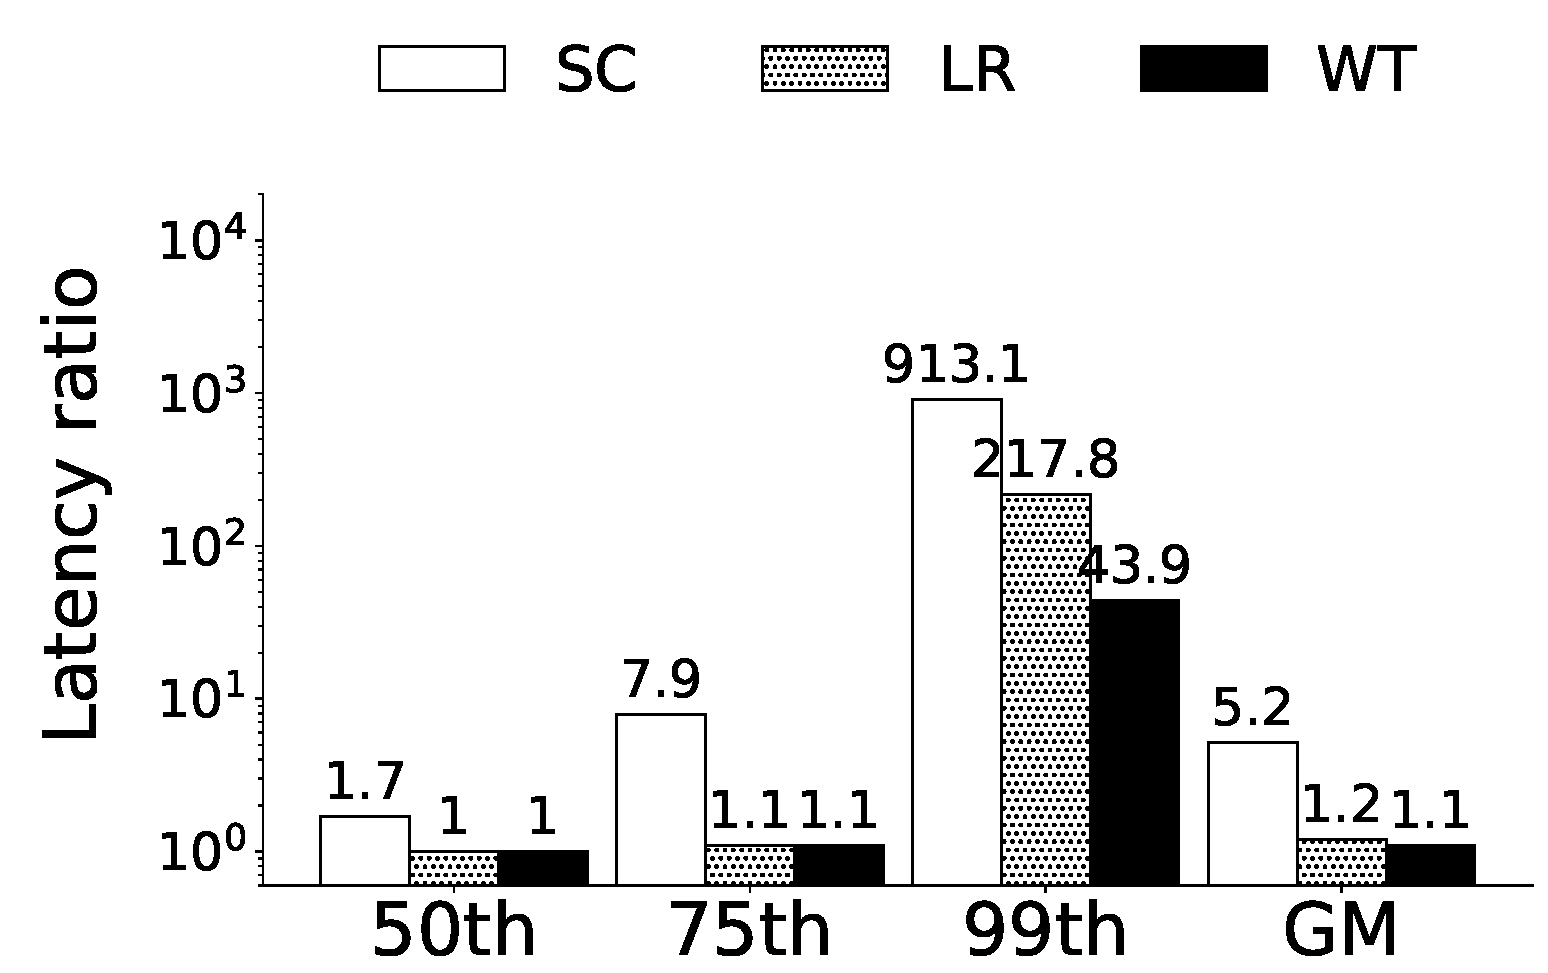
\includegraphics[width=\linewidth]{chapters/slabcity/figs/time_Calcite_250K.pdf}
\end{minipage}\\[8pt]
\begin{minipage}[t]{.48\linewidth}\centering
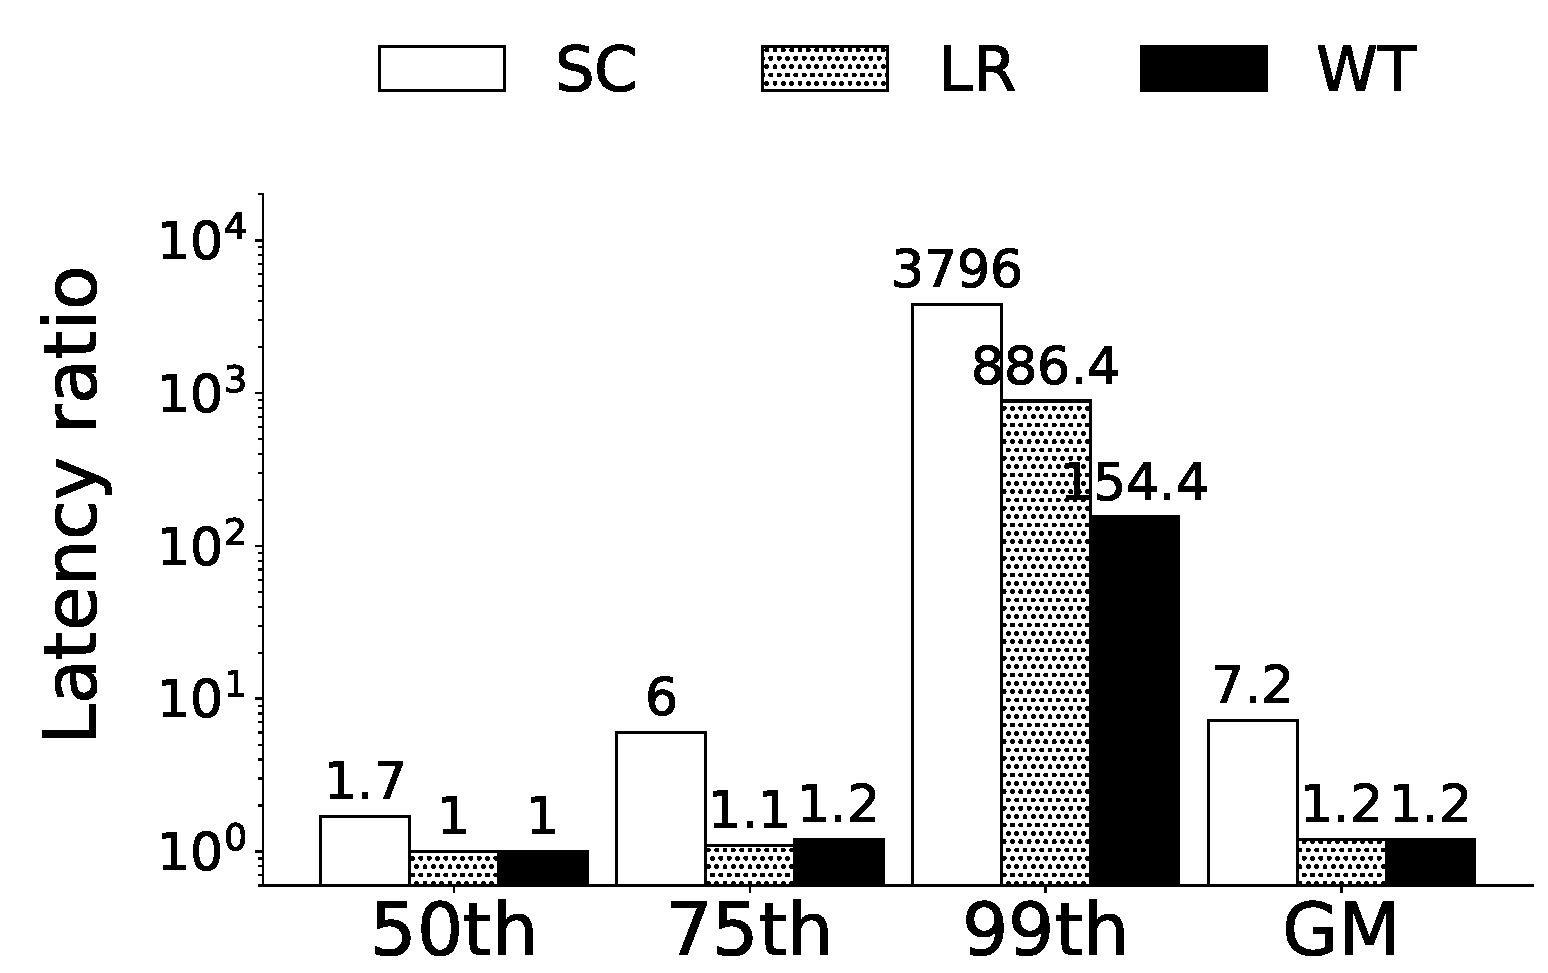
\includegraphics[width=\linewidth]{chapters/slabcity/figs/time_Calcite_1M.pdf}
\end{minipage}\hfill
\begin{minipage}[t]{.48\linewidth}\centering
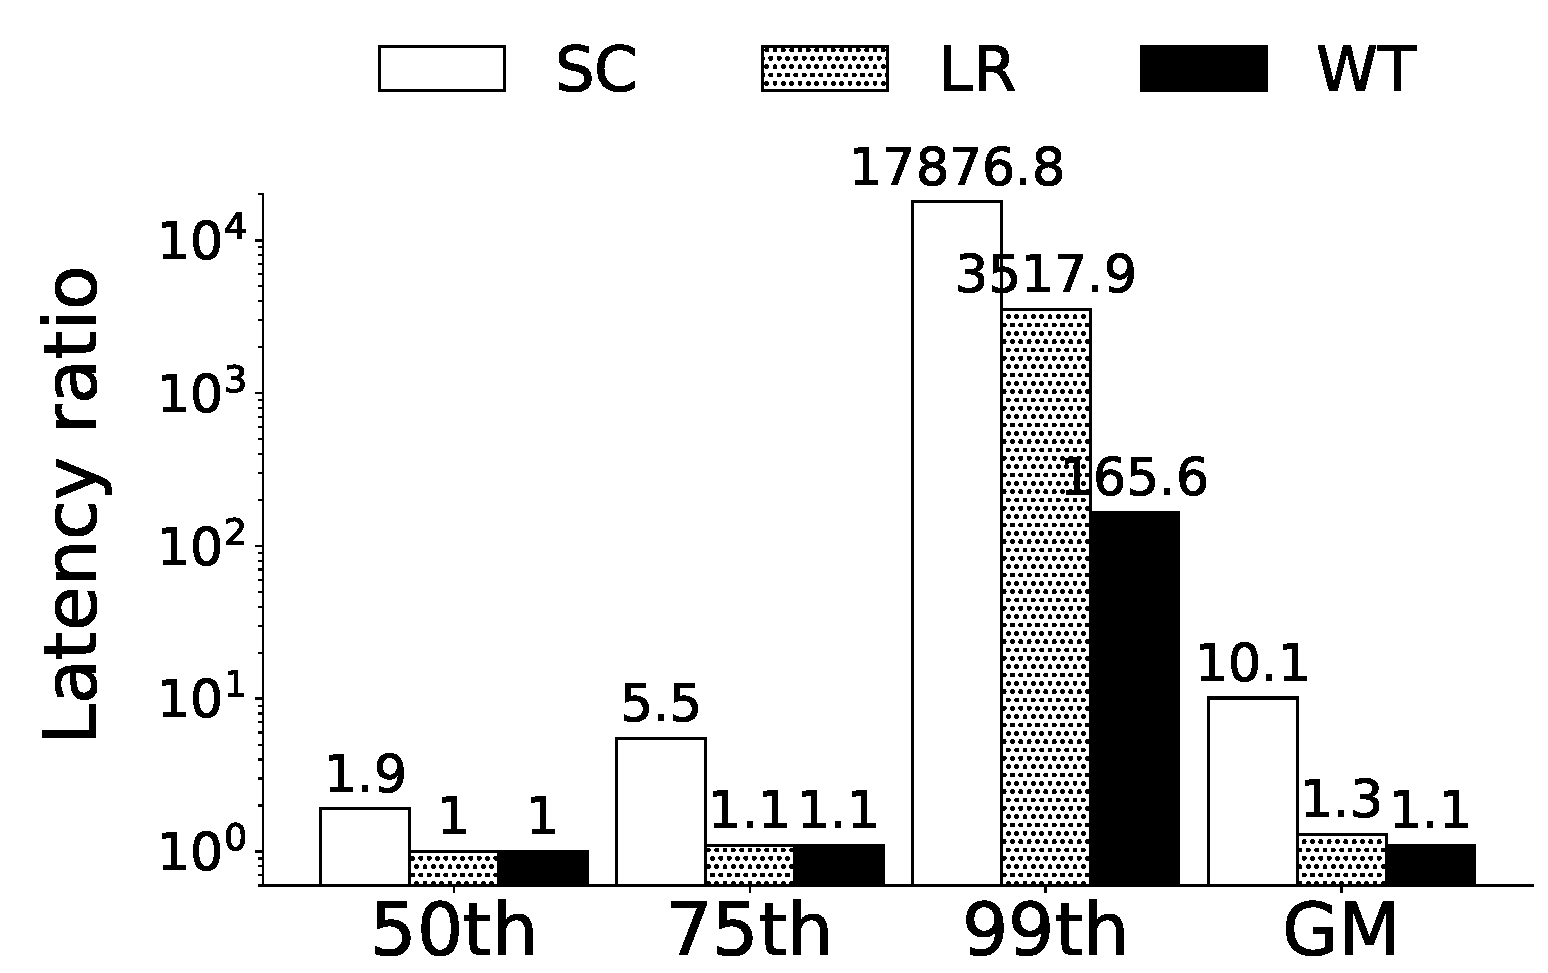
\includegraphics[width=\linewidth]{chapters/slabcity/figs/time_Calcite_4M.pdf}
\end{minipage}
\caption*{\small (b) Latency reduction: top right is on 250K, bottom left is on 1M, and bottom right is on 4M. ``GM'' means geometric mean.}
\label{slab:fig:calcite-reduction-latency}
\caption{\barzanrev{Calcite results across all data sizes with uniform distribution.}}
\label{slab:fig:calcite-results}
\end{figure*}




Our experiments are designed to answer the following questions:

\begin{itemize}[leftmargin=*]  \setlength\itemsep{2pt}
\item 
\textbf{Coverage:} 
How does $\toolname$'s \emph{coverage} compare against that of state-of-the-art query rewriting techniques? 
That is, which technique can optimize more queries? 
(Section~\ref{slab:sec:q1-coverage}) 
\item 
\textbf{Query latency reduction:}
How does $\toolname$ compare to state-of-the-art query rewriters in terms of the efficiency of the generated queries? 
That is, for input queries that can be rewritten, which technique leads to faster queries? 
(Section~\ref{slab:sec:q2-reduction})
 
\item
\textbf{Ablation study:} How important are various ideas in \slabcity? 
(Section~\ref{slab:sec:ablation})

\end{itemize}



\subsection{Experimental Setup}
%In what follows, we describe our workloads, data generation method, baselines, and experiment environment.

\head{Testbed}
All of our experiments (including running \toolname and baselines as well as executing queries) are conducted on Amazon EC2 r5.large instances,
% \barzan{is it EC2? if so then mention the size, eg. 2XL or something like that}
with 16GB RAM, 200GB gp2 SSD and Xeon E5-2686 v4 CPU running Ubuntu 22.04.
We use PostgreSQL 12.13.

\head{Workloads} 
{We use a wide range of different workloads:}
\begin{itemize}[leftmargin=*]
\item 
\textbf{LeetCode.} 
These are SQL queries, written by actual developers to solve different problems on LeetCode~\cite{leetcode}. 
Specifically, we first crawled \emph{all publicly available} SQL queries accepted by LeetCode as ``correct'' solutions. However, a number of them are actually incorrect due to missing tests on LeetCode. Hence, we manually filtered out as many incorrect queries as we could. 
In the end, we were left with a curated suite of 1131 queries overall. 
% Our dataset contains queries that solve a wide range of tasks (see some examples from Section~\ref{slab:sec:motivating-example}). 
%Then, we grouped these queries based on the LeetCode problem they are solving. 
%For each problem, we were left with dozens of correct queries that are all \emph{semantically equivalent} but \emph{syntactically distinct}.
Some of these solutions are poorly-written and therefore slow-running (which we hypothesize were authored by SQL novices) -- this makes  our LeetCode dataset especially 
valuable for evaluating query rewriting techniques. 
We also formalized the schemas and integrity constraints for all LeetCode tasks. 
%based on the description from the LeetCode website. 

\begin{comment}
\cancut{Overall, the queries were quite diverse and non-trivial. On our 10M database, \todo{xx} queries do not terminate within 10 hours, and \todo{xx} queries take at least \todo{xx} seconds to finish. Even on our smallest database with 100K rows, \todo{xx} queries take more than \todo{xx} seconds.}
\end{comment}



\item 
\textbf{Calcite.}
Our second workload is constructed from the Calcite's \emph{optimization rules} test suite~\cite{calcite-test-suite}, which is used in prior work~\cite{wetune} for evaluating query rewriting. We include all 794 queries. %in our experiments.
%The Calcite project also includes the schema and integrity constraints.


\item 
\barzanrev{\textbf{TPC.}
Finally, we also use queries from the standard TPC-H~\cite{tpc-h} and TPC-DS~\cite{tpc-ds} workloads.}
\end{itemize}


\head{Data generation} 
We generate large databases for each workload. 
For \leetcode, we use three data sizes (100K, 1M, and 10M). For \calcite, we use 250K, 1M, and 4M (4M is the largest data size that can fit in 16G memory). 
For both workloads, we follow prior work~\cite{wetune} and use \barzanrev{two different data distributions: uniform and Zipfian
% \barzan{isn't Zipfian capitalized everywhere?} \jie{also used in WeTune paper. And they also use the skewed parameter of 1.25. Do we need to mention it?}
(with a skewed parameter of 1.25, as used in \cite{wetune}).}
% \barzan{is 1.25 skeweed enough?} \jie{see above. Yes, I believe it is skewed enough}
We also make sure the generated data meets the integrity constraints. 
\barzanrev{For TPC-H and TPC-DS workloads, we use their official data generation script with the same scale factor as in $\learnedrewrite$~\cite{LR} (which is 1, meaning 1G data size).}





\head{Baselines}
We compare $\toolname$ against two state-of-the-art rule-based query rewriting techniques: 
\begin{itemize}[leftmargin=*]
\item
\textbf{\learnedrewrite} (or \LR, VLDB 2022~\cite{LR,LR-source-code}) is a state-of-the-art \emph{rule-based} query rewriter which uses Monte Carlo Tree Search to guide the rule-based rewriting process. In particular, \LR uses rewrite rules from \calcite and was shown to outperform multiple existing techniques from prior work~\cite{begoli2018apache,pirahesh1992extensible}.
\item 
\textbf{\wetune} (or \WT, SIGMOD 2022~\cite{wetune,WT-source-code}) is the state-of-the-art automated query rewrite rule generator. It had discovered dozens of new rules, previously missing from existing rule-sets. These new rules were shown to lead to new optimizations previously not considered by existing systems (such as MS SQL Server).  
\end{itemize}




\begin{comment}
\rui{All of our experiments are conducted on AWS EC2 
instances (r5.large type, with 16GB RAM, 200GB disk, Xeon E5-2686 v4 CPU, running Ubuntu 22.04 and PostgreSQL 12.13). We launched instances using the same Amazon Machine Image with testing databases loaded to ensure the same experiment setups over all instances. We collected cost by first running VACUUM ANALYZE and running EXPLAIN on queries on a single machine. For the running time, we partitioned the queries to collect their running time on multiple instances parallelly. For LeetCode experiments, we partitioned queries using problem ID so that all queries corresponding to the same problem id are run on the same instance. For Calcite experiments, we ensured that outputs that correspond to the same test were run on the same instances.  Between each run, we restarted the PostgreSQL service and cleared the cache.}
\end{comment}





%ta inja

\subsection{Coverage}
\label{slab:sec:q1-coverage}

This section reports the number of queries from each workload that \toolname can optimize, and compare it with baselines.


\head{Setup}
Given each query $\inputquery$ (and the corresponding schema) from each workload, we run \toolname (using a 5-second timeout) and obtain an output query $\query$. 
Then, we check whether or not $\query$ indeed optimizes $\inputquery$ in terms of latency: if $\query$ has a smaller latency than $\inputquery$, we say $\query$ optimizes $\inputquery$. 
%\barzan{this def should  come much earlier in the paper} %\xinyu{I added this to section 2.}
%Similarly, $\query$ optimizes $\inputquery$ in terms of latency, if $\query$ has a smaller execution time than $\inputquery$. 
We run each query (both input and rewritten queries) 3 times and take their average as the final latency value.
%the first run serves as warm-up whereas the average of the next 3 runs is used as the final latency value. 
Before each run, we restart the PostgreSQL service and clear the database cache. 
We use 10 hours as the timeout; output queries that do not terminate before timeout are marked as ``not optimized''. 
The same setup is used for the baselines. 

\vspace{5pt}
\evalfinding{\emph{\toolname can optimize more queries across different workloads.}}




\begin{table}[!t]
%\small 
\footnotesize
\caption{\barzanrev{\small LeetCode and Calcite results with Zipfian distribution.}}
\vspace{-8pt}
\centering
\setlength{\tabcolsep}{2pt}
\def\arraystretch{1.1}
\begin{tabular}{  c | r r r | r r r | r r r | r r r }
\toprule
& \multicolumn{6}{c|}{Coverage (\# of queries)} 
& \multicolumn{6}{c}{Latency ratio (geometric mean)} 
\\ 
\midrule
& \multicolumn{3}{c|}{LeetCode} 
& \multicolumn{3}{c|}{Calcite} 
& \multicolumn{3}{c|}{LeetCode} 
& \multicolumn{3}{c}{Calcite} 
\\ 
& 100K & 1M & 10M 
& 250K & 1M & 4M 
& 100K & 1M & 10M 
& 250K & 1M & 4M 
\\ 
\midrule
$\toolname$
& \textbf{318} & \textbf{269} & \textbf{186}
& {\textbf{101}} & {\textbf{99}} & {\textbf{96}}
& \textbf{3.1x} & \textbf{2.7x} & \textbf{2.2x}
& {\textbf{5.4x}} & {\textbf{8.8x}} & {\textbf{12.8x}}
\\ 
$\LR$
& 262 & 243 & 154  
& {95} & {94} & {86} 
& 1.1x & 1.2x & 1x
& {1.2x} & {1.3x} & {1.3x}

\\ 
$\WT$
& 24 & 23 & 24  
& {20} & {23} & {18}
& 1.4x & 1.6x & 1.6x
& {1.2x} & {1.2x} & {1.2x}
\\ 
\bottomrule
\end{tabular}
%\vspace{5pt}

\label{slab:tab:zipfian-results}
\vspace{-15pt}
\end{table}




\head{Results}
Figure~\ref{slab:fig:leetcode-results}(a) and Figure~\ref{slab:fig:calcite-results}(a) present the coverage results for all techinques (including $\toolname$ and baselines) across LeetCode and Calcite workloads (using a uniform distribution). 
For example, looking at Figure~\ref{slab:fig:leetcode-results}(a), for 10M, \toolname can optimize 222 input queries, whereas $\learnedrewrite$ and $\wetune$ can only 
optimize 132 and 20 queries, respectively. 
\barzanrev{We also note that since $\toolname$'s checker can fully verify only a subset of its output queries, we manually inspected all the remaining queries that only pass the tester and bounded verifier (see Section~\ref{slab:sec:eval:discussion} for a detailed discussion on the limitation of full verification) and confirmed the optimizations included in our results are indeed correct} (i.e., all input-output query pairs are equivalent).
%\barzanrev{Although the checker can offer full verification for only a subset of the output queries, we manually inspect and confirm all our optimizations are indeed correct} (i.e., all input-output query pairs are equivalent). 
\barzanrev{For the Zipfian distribution, we obtain similar results, as shown in Table~\ref{slab:tab:zipfian-results}.}
Overall, $\toolname$ significantly outperforms existing rule-based systems, highlighting the superiority of a whole-query synthesis-based approach.


\barzanrev{For the TPC-H workload, $\toolname$ is able to optimize 2 (out of 22) input queries (\#17 and \#20) in less than 5 seconds. $\LR$ is able to optimize the same two queries, while $\WT$ cannot optimize any.
The TPC-DS queries are far more complex, but $\toolname$ can still optimize three queries (\#1, \#30 and \#81) within 5 seconds. $\LR$ can optimize two (\#1, \#30) but $\LR$'s output queries are much slower than $\toolname$'s. Again, $\WT$ is not able to optimize any.}



\head{Discussion}
The gap between \toolname's coverage and baselines' on LeetCode is much higher than that on Calcite: we believe this highlights the usefulness of our LeetCode dataset and the advantage of our synthesis-based technique over rule-based ones in optimizing new query patterns. 
In particular, LeetCode has more queries that are larger and use more aggregation and window functions than those in Calcite. 
\barzanrev{While $\toolname$'s coverage is considerably higher than all baselines, there are still 
some queries covered by baselines and not covered by $\toolname$.
%While rare (\todo{??\% for)}, 
Some of these queries involve operators (e.g., coalesce) that are not yet supported by our prototype. 
Another reason has to do with our 5s timeout. 
Our plan for future improvement of our prototype (e.g., supporting more operators and optimizing the performance such as by parallelizing the search) should help with both reasons.}
%Another reason is our 5s timeout. 
%Our plans for future improvement of our implementation (supporting more operators and improving the efficiency) should help with both reasons.}





\begin{comment}
    

\todo{if above looks good, we can comment out below. }
\jierevision{There are two primary explanations as to why our tool may be unable to optimize for certain queries, while baselines can. The first reason is that baselines rewrite the input query by employing operators (e.g., $\sqlcoalescecolor$) that are not available in our DSL. The second reason is that sometimes our score function fails to capture the similarity in semantics of different dataflows and hence assigns some promising candidates with lower scores than expected. As a result, they cannot be found within 5s timeout. Table~\ref{slab:tab:Q11-Q12} shows queries finding the team size of each employee. \slabcity did not capture the relationship between $\sqloncolor \ e1.team = e2.team$ and $\sqlgroupbycolor \ team$ and failed to find the optimal query. To address this issue, one solution is to adjust the score function to take this relationship into account. However, it is important to note that incorporating more dataflows will inevitably lead to increased search time, which is a tradeoff that needs to be carefully balanced.} 

\begin{table}[!t]
\small 
\begin{tabular}{|c|c|}
\hline
 $\query_{11}$

 & 
  % \\
  %             \hspace{2em} 
 \makecell[l]{\sqlselectcolor \  e1.employee\_id, \sqlcountcolor(e2.employee\_id) \sqlascolor s\\
              \sqlfromcolor employee \sqlascolor e1 \sqljoincolor employee \sqlascolor e2 \sqloncolor e1.team = e2.team\\
              $\sqlgroupbycolor$ e1.employee\_id
              }  
\\
\hline
$\query_{12}$
&
 \makecell[l]{ \sqlselectcolor e1.employee\_id, e2.s, \\ \sqlfromcolor employee \sqlascolor e1 \sqljoincolor \\
 \hspace{0.5em} (\sqlselectcolor team, \sqlcountcolor(*) \sqlascolor s \sqlfromcolor employee \sqlgroupbycolor \ team) \sqlascolor e2 \\ \hspace{0.5em} \sqloncolor e1.team = e2.team}
 
  \\
 \hline
\end{tabular}
\vspace{5pt}
\caption{\jierevision{$\query_{11}$ is human-written. $\query_{12}$ is the optimal form.}}
\vspace{-20pt}
\label{slab:tab:Q11-Q12}
\end{table}

\end{comment}


\subsection{Query Latency Reduction}
\label{slab:sec:q2-reduction}


In this section, we compare the performance of queries synthesized by $\toolname$  with those generated by (rule-based) baselines. Higher coverage (Section~\ref{slab:sec:q1-coverage}) means $\slabcity$ can optimize more queries, 
but does it also lead to better (i.e., faster) queries than baselines?

\head{Setup}
We use the same setup as in Section~\ref{slab:sec:q1-coverage} and measure the reduction ratio in query latencies across each technique's output queries. 
For example, given $\inputquery$ and its corresponding output query $\query$ synthesized by \toolname, a latency reduction of 5x means $\query$ is 5x faster than $\inputquery$. 
We still use 10 hours as the timeout --- in case of a timeout, we use 10 hours as the latency; however, if both $\inputquery$ and $\query$ time out, we do not include this data point. 
%Latency reduction ratios for baselines are measured in the same way.

\vspace{5pt}
\evalfinding{\emph{\toolname generates faster queries across different workloads.}}


\head{Results}
We present the latency reduction results for LeetCode and Calcite workloads (using a uniform distribution) in Figure~\ref{slab:fig:leetcode-results}(b) and Figure~\ref{slab:fig:calcite-results}(b). 
For example, looking at Figure~\ref{slab:fig:leetcode-results}(b), for 10M (rightmost figure), on average, $\toolname$ achieves a 50.3x latency reduction ratio \emph{across all output queries}, whereas $\LR$ is 1.4x and $\WT$ is 12x. 
\barzanrev{We also report additional statistics: median (50th) and 75th percentiles.}
As we can see, $\toolname$ always outperforms baselines by a significant margin across both workloads and for all data sizes. 
\barzanrev{For output queries that can be covered (i.e., optimized) by $\toolname$,} the median is as high as 1.9x for LeetCode and 2.2x for Calcite.
% \barzan{what does it mean for median to be up to? shouldn't median be a single number?
% maybe we can reword to `as high as` instead of up to}
% \xinyu{because we have multiple data sizes.}
% \barzan{the following is confusing: we say on the other hand if we said on the one hand earlier which we didn't early. what are we trying to say in the next sentence? } \xinyu{we can remove OTOH}
% On the other hand, 
\barzanrev{For the Zipfian distribution, $\toolname$ also outperforms all baselines; see Table~\ref{slab:tab:zipfian-results} for more details.}

\barzanrev{For TPC-H, $\toolname$ and $\LR$ achieve similar latency speed-ups (both by more than an order of magnitude). 
For TPC-DS, $\toolname$ can optimize one query that $\LR$ is not able to optimize. For the two TPC-DS queries that both can optimize, $\toolname$ outputs faster queries compared to $\LR$'s. For all three TPC-DS queries, $\toolname$ can speed-up the original queries by at least one order of magnitude.}

%\xinyurevision{\todo{For TPC-H, $\toolname$ and $\LR$ produce queries with very similar latency reduction ratios. However, for TPC-DS, $\toolname$'s output queries are significantly faster. In particular, it achieves a {1034x} reduction for query \#1 and $\LR$ is {189x}. For \#30, $\toolname$ is {113x} and $\LR$ is {26x}. \ruirevision{For \#81, $\toolname$ is 364x and $\LR$ can not optimize.}}}


{\head{Discussion}
Similar to Section~\ref{slab:sec:q1-coverage}, \toolname's margins of improvement on LeetCode are even more significant than on Calcite, which we believe is due to the same reasons mentioned earlier: 
existing rule-based systems and \learnedrewrite's rule-set are specifically designed based on Calcite queries and LeetCode is a useful dataset to evaluate query rewriters. 
Careful readers may observe that \toolname's reduction on LeetCode 10M is lower than that on 1M.
This is due to 15 input queries (all from problem \#1308) which do not terminate within 10 hours on both sizes. Surprisingly, \toolname is able to optimize these queries: the fastest output query terminates in 3 seconds on 1M but takes more than 30 seconds on 10M. 
As we used 10 hours as the latency for the timed-out input query in both cases, this makes the reduction on 10M lower than that on 1M.}




\begin{table}[!t]
%\small 
\footnotesize
\caption{\small Time breakdown on average and other statistics.}%Bottom:  other statistics (e.g., the average number of queries enumerated).}
\vspace{-8pt}
\centering
\setlength{\tabcolsep}{3pt}
\def\arraystretch{1.5}
\begin{tabular}{  R{180pt} | r  r   }
\toprule
\% of time spent on 
& LeetCode
& Calcite
%& TPC-H 
%& TPC-DS 
\\ \midrule
{query search (line~\ref{slab:alg:toplevelalg:forloop})} 
& {37.4\%}
& {6.9\%} 
%& \ruirevision{48.0\%}
\\ 
{checking against counterexamples (line~\ref{slab:alg:toplevelalg:satisfycounterexample}}) 
& {10.8\%}
& {0.9\%}
%& \ruirevision{2.9\%}
\\ 
{equivalence  checking (line~\ref{slab:alg:toplevelalg:checkequiv}})
& {51.4\%}
& {92.2\%}  
%& \ruirevision{51.0\%}
\\ 
%\emph{\% of time on testing} 
%& 32.6\% 
%& 65.5\% 
%\\ 
%\emph{\% of time on verification} 
%& 23.6\% 
%& 31.6\% 
%\\ \midrule 
{performance ranking (line~\ref{slab:alg:toplevelalg:checkfaster})} 
& {0.4\%} 
& {0.1\%} 
%& \ruirevision{0.1\%}
\\ \midrule \midrule 
{avg \# of queries enumerated}
& {437} 
& {104}
%& \ruirevision{216}
\\ 
{avg \# of counterexamples generated}
& {1.4}
& {1.2}
%& \ruirevision{1}
\\ 
{avg \# of equivalent queries synthesized}
& {66}
& {15} 
%& \ruirevision{32}
\\ \bottomrule
\end{tabular}

\vspace{-12pt}
\label{slab:tab:time-breakdown}
\end{table}




\subsection{Detailed Analysis and Ablation Study}
\label{slab:sec:ablation}

%In this section, we analyze the time that is spent on different steps of \slabcity. We also perform a few ablation studies to measure the impact of various design decisions we have made in \slabcity.


\begin{comment}
    

\begin{table}[!t]
%\small 
\footnotesize
\centering
\setlength{\tabcolsep}{2pt}
\def\arraystretch{1.1}
\begin{tabular}{  c | r r | r r  }
\toprule
& \multicolumn{2}{c|}{LeetCode} 
& \multicolumn{2}{c}{Calcite} 
%& \multicolumn{2}{c|}{TPC-H} 
%& \multicolumn{2}{c}{TPC-DS} 
\\ 
& median 
& max 
& median 
& max 
%& median 
%& max 
%& median 
%& max 
\\ 
\midrule
$\toolname$
& {0.84} & {4.84} & 
 {0.74}	&  {4.81}	
 %& \ruirevisiontbd{4.15}  &  \ruirevisiontbd{4.58}	 &  \ruirevisiontbd{5.03}		& \ruirevisiontbd{5.74}
\\ 
$\learnedrewrite$
& 0.03 & 0.73 & 0.25	& 3.75	 
%& 0.25 & 	1.58 & 	2.48	& 25.51 
\\ 
$\wetune$
& 0.24	& 0.46 &	0.001	& 0.17	
%& 0.36	& 0.36	& NA &	NA 
\\ 
\bottomrule
\end{tabular}
%\vspace{5pt}
\caption{{\small Running time statistics to generate rewrites (in seconds). For $\toolname$, we report the time when an output query (synthesized using 5-second timeout) is found.}}
\label{slab:tab:running-time-stats}
\vspace{-20pt}
\end{table}

\end{comment}



\begin{table}[!t]
\centering
\footnotesize
\centering
\setlength{\tabcolsep}{6pt}
\def\arraystretch{1.5}
\caption{\small Running time statistics to generate rewrites (in seconds).For $\toolname$, we report the time when an output query (synthesized using 5-second timeout) is found.}
\vspace{-5pt}
\begin{tabular}{  c | r r | r r  }
\toprule
& \multicolumn{2}{c|}{LeetCode} 
& \multicolumn{2}{c}{Calcite} 
%& \multicolumn{2}{c|}{TPC-H} 
%& \multicolumn{2}{c}{TPC-DS} 
\\ 
& median 
& max 
& median 
& max 
%& median 
%& max 
%& median 
%& max 
\\ 
\midrule
$\toolname$
& {0.84} & {4.84} & 
 {0.74}	&  {4.81}	
 %& \ruirevisiontbd{4.15}  &  \ruirevisiontbd{4.58}	 &  \ruirevisiontbd{5.03}		& \ruirevisiontbd{5.74}
\\ 
$\learnedrewrite$
& 0.03 & 0.73 & 0.25	& 3.75	 
%& 0.25 & 	1.58 & 	2.48	& 25.51 
\\ 
$\wetune$
& 0.24	& 0.46 &	0.001	& 0.17	
%& 0.36	& 0.36	& NA &	NA 
\\ 
\bottomrule
\end{tabular}

\label{slab:tab:running-time-stats}
\end{table}

\begin{table}[!t]
% 
%
\centering
\footnotesize
\centering
\setlength{\tabcolsep}{2pt}
\def\arraystretch{1.1}
\caption{{\small Coverage (\# of queries) and geometric mean of latency reduction: using \texttt{EXPLAIN} vs. using exact latencies.}}
\vspace{-5pt}
\begin{tabular}{  c | r r r | r r r | r r r | r r r }
\toprule
& \multicolumn{6}{c|}{Coverage (\# of queries)} 
& \multicolumn{6}{c}{Latency ratio (geometric mean)} 
\\ 
\cmidrule{2-13}
& \multicolumn{3}{c|}{LeetCode} 
& \multicolumn{3}{c|}{Calcite} 
& \multicolumn{3}{c|}{LeetCode} 
& \multicolumn{3}{c}{Calcite} 
\\ 
& 100K & 1M & 10M 
& 250K & 1M & 4M 
& 100K & 1M & 10M 
& 250K & 1M & 4M 
\\ 
\midrule
w/ \texttt{EXPLAIN} 
& 315 & 301 & 222  & 106 & 101 & 97 
& {2.7x} & {2.2x} & {2.1x}  & {5.2x} & {7.2x} & {10.1x} 
\\ 
w/ exact latencies 
& {401} & {373} & {351}  & {121} & {117} & {112} 
& {2.9x} & {2.6x} & {2.2x}  & {4.8x} & 6.7x & {10.4x} 
\\ 
\bottomrule
\end{tabular}

\label{slab:tab:exact-latencies}
\end{table}


\head{Time breakdown}
Table~\ref{slab:tab:time-breakdown} shows the breakdown of how much time on average \toolname spends in each component (such as search and equivalence checking) and other statistics (such as the average number of queries generated during synthesis). 
In general, query equivalence checking (including both testing and verification) takes the majority of the time. 


\barzanrev{\head{Synthesis efficiency}
While $\toolname$ uses a 5s \emph{timeout}, many of its output queries are discovered 
much earlier.
Specifically, {58\%} of its output queries (generated using 5s timeout) are found within {1} second. 
In the words, the actual synthesis time to find the output query is shorter. 
Table~\ref{slab:tab:running-time-stats} presents the median and max of $\toolname$'s actual synthesis time for LeetCode and Calcite queries that $\toolname$ can rewrite.
As expected, rule-based approaches are generally faster, though $\LR$'s max time on Calcite is much slower. 
For TPC-H and TPC-DS, $\toolname$ takes 4-5 seconds for all queries it can optimize.}
%\xinyurevision{In comparison, $\LR$  is significantly slower: it takes up to 25 seconds for TPC-DS.}}














\begin{comment}

===== 
\xinyu{below is old stuff, but once we have Table 6 filled, will move something from below to above..}

As we can see, query testing takes more than 60\% of the total time, while verification takes more than 30\%. 
Note that this is not because our tester is slower than the verifier, but rather because the tester is run before verifier and disproved many inequivalent queries before they were sent to the verifier. 
For instance, on LeetCode 10M, an average of \rui{do you mean counter examples can not reject?} queries were sent to our tester, out of which only a dozen \rui{14.22} of queries were not disproved. 
On the other hand, our query search component tends to be quite fast. In particular, for LeetCode 10M, on average, a total of \rui{93 our algorithm ensures these queries are syntactically different and grammarly correct, so the number here is small, but high quality} queries can be searched within the 5-second time limit. Using \texttt{EXPLAIN} to collect cost estimates takes no time, since eventually only a handful of equivalent queries were synthesized --- e.g., for LeetCode 10M, on average, \rui{13.59} queries were ranked. 
\end{comment}



\begin{comment}


\begin{table}[!t]
\small 
\centering
\setlength{\tabcolsep}{3pt}
\def\arraystretch{1.2}
\begin{tabular}{ | r | c c c | c c c | }
\hline 
& \multicolumn{3}{c|}{LeetCode} 
& \multicolumn{3}{c|}{Calcite} 
\\ 
& 100K & 1M & 10M 
& 250K & 1M & 4M 
\\ \hline 
\emph{Query Search}
& 5.3\% & 5.4\% & 5.2\% & 0.7\% & 0.9\% & 0.9\%
\\ 
\emph{Equivalence Testing} 
& 61.4\% & 60.0\% & 60.3\%  & 66.1\% & 67.0\% & 67.3\%\\ 
\emph{Equivalence Verification} 
& 33.0\% & 34.3\% & 34.2\%  & 33.0\% & 32.0\% & 31.7\%\\ 
\emph{Performance Ranking} 
& 0.3\% & 0.3\% & 0.3\%  & 0.1\% & 0.1\% & 0.1\%
\\ \hline 
\end{tabular}
\vspace{5pt}
\caption{$\toolname$ time breakdown.}
\label{slab:tab:time-breakdown}
\end{table}

\end{comment}


\head{Impact of CEGIS}
How beneficial is the use of CEGIS? That is, if we do not re-use counterexamples when disproving queries, how inefficient would \toolname become? 
%In general, program synthesis is known to be prohibitively slow without using counterexamples~\cite{solar2008program}. To validate this in the context of synthesis-based query rewriting, 
%For instance, 
For LeetCode, with CEGIS, on average, $\toolname$ can search {437} queries in 5 seconds, where {1.4} counterexamples are generated; however, without re-using these examples, it can only search 175 queries on average within the same amount of time. 
This is because the tester spends extra time generating new counterexamples which are later dropped, but clearly they can be re-used to disprove other queries.  
This validates the observation made in prior work that CEGIS helps boost efficiency~\cite{solar2008program}. 

%generate \tofix{the examples from scratch.}\barzan{can we instead say `to disprove the same queries'?}
%This validates the observation made in other domains that CEGIS is critical for synthesis efficiency~\cite{solar2008program}. 




\head{Impact of query testing}
It is critical to reduce the frequency of invoking query verification. 
For instance, for LeetCode, on average our tester can disprove several dozens of queries within 1 second, whereas the verifier typically can handle at most a couple of queries within the same amount of time.
%A variant of \slabcity that invokes the query verifier to disprove \emph{every} candidate query (rather than always running the tester first)


\head{Impact of using dataflows to guide search}
A variant of $\slabcity$ that uses a naive search algorithm (that enumerates queries based on query size) was not able to optimize any of our input queries within 5 seconds. 
This highlights the importance of using dataflows to significantly accelerate query synthesis. 

\head{Impact of using cost estimates for ranking}
\texttt{EXPLAIN} is known to give inaccurate cost estimates. 
We study a variant of \slabcity where, instead of \texttt{EXPLAIN}, we  use the actual latency for each query (by running it against the database). 
While this variant is clearly impractical, it helps us understand how much \slabcity could be improved if we had access to a perfect predictor that could give the exact latency values. 
Table~\ref{slab:tab:exact-latencies} compares $\toolname$ w/ exact latency against our current $\toolname$ w/ \texttt{EXPLAIN} in terms of coverage; Table~\ref{slab:tab:exact-latencies} compares them in terms of latency reduction. 
In general, using exact latencies yields slightly higher coverage and latency reduction ratios, which is expected as that is the perfect predictor. 
However, we notice that using \texttt{EXPLAIN} to estimate query latency gives very close results and we believe this is a reasonable trade-off. 



\begin{comment}
    

\begin{table}[!t]
\footnotesize
\centering
\setlength{\tabcolsep}{3pt}
\def\arraystretch{1.1}
\begin{tabular}{  c | rrr | rrr  }
\toprule
& \multicolumn{3}{c|}{LeetCode} 
& \multicolumn{3}{c}{Calcite} 
%& \multirow{2}{*}{\rotatebox{0}{TPC-H}}
%& \multirow{2}{*}{\rotatebox{0}{TPC-DS}} 
\\ 
& 100K & 1M & 10M 
& 250K & 1M & 4M 
%& & 
\\ \midrule
w/ \texttt{EXPLAIN} 
& 315 & 301 & 222  & 106 & 101 & 97 
%& \ruirevision{2}  & \ruirevision{2}
\\ 
w/ exact latencies 
& {401} & {373} & {351}  & {121} & {117} & {112} 
%& \ruirevision{2}  & \ruirevision{2}
\\ \hline 
\end{tabular}
\vspace{5pt}
\caption{\small Coverage \ruirevision{(\# of queries)}: using \texttt{EXPLAIN} vs. using exact latencies.}
\label{slab:tab:oracle-coverage}
\vspace{-20pt}
\end{table}


\begin{table}[!t]
\footnotesize
\centering
\setlength{\tabcolsep}{2pt}
\def\arraystretch{1.1}
\begin{tabular}{  c | rrr | rrr }
\toprule
& \multicolumn{3}{c|}{LeetCode} 
& \multicolumn{3}{c}{Calcite} 
%& \multirow{2}{*}{\rotatebox{0}{TPC-H}}
%& \multirow{2}{*}{\rotatebox{0}{TPC-DS}}
\\ 
& 100K & 1M & 10M 
& 250K & 1M & 4M 
%& 
%& 
\\ \midrule   
w/ \texttt{EXPLAIN} 

& {2.7} & {2.2} & {2.1}  & {5.2} & {7.2} & {10.1} 
%& \ruirevision{1429.4} & \ruirevision{341.6}

\\ 
w/ exact latencies 

& {2.9} & {2.6} & {2.2}  & {4.8} & 6.7 & {10.4} 
%& \ruirevision{1429.4} & \ruirevision{341.6}

\\ \bottomrule
\end{tabular}
\vspace{5pt}
\caption{\small Geometric mean of latency reduction: using \texttt{EXPLAIN} vs. using exact latencies.}
\label{slab:tab:oracle-reduction1}
\vspace{-20pt}
\end{table}

\end{comment}



\head{Percentage of fully verified rewrites}
A subset of $\slabcity$'s rewrites can be \emph{fully} verified by the {full} verifier --- meaning queries in this subset are guaranteed to be equivalent to their corresponding input queries, \emph{for all possible inputs}.
For example, for LeetCode 100K, {17\%} of the queries can be fully verified by $\cosette$ and $\spes$. We explain the implications in the next Section~\ref{slab:sec:eval:discussion}.


\subsection{Discussion}
\label{slab:sec:eval:discussion}


\barzanrev{While $\toolname$'s percentage of fully verified rewrites (about 17\%) might sound low, one 
must remember that the vast majority of rewrite rules in existing rule-based techniques are not fully verified~\cite{chu2017hottsql,chu2018axiomatic} and rely on human verification, which is error-prone. In fact, a considerable fraction (about 5\%) of rewrites generated by $\learnedrewrite$ using the Calcite rule-set were proved  incorrect by $\toolname$'s checker. %Further inspection also revealed multiple buggy rewrite rules (confirmed by Calcite developers~\cite{calcite-bug-1,calcite-bug-2,calcite-bug-3}). 
In contrast, all of $\toolname$'s rewrites pass the checker. 
Even those few prior approaches that do offer formal guarantees, they do so for a much smaller 
%percentage
{number}
of queries than $\toolname$ (e.g., 7 queries in the FGH work~\cite{wang2022optimizing}). 
%vs. \xinyurevision{more than 50 in $\toolname$}). 

In reality, the percentage of rewrites that can benefit from full verification has little impact on $\toolname$'s specific use case, which, as explained in Section~\ref{slab:sec:intro}, is any scenario where a query is rerun many times, such as BI dashboard queries. 
In such scenarios,  many rewrites receiving a ``bounded verification'' flag is not a hindrance since the human inspection can be performed at the time of defining the queries and before deploying the dashboard to production.}

\barzanrev{Furthermore, $\toolname$'s use of a tester and a bounded verifier in conjunction with full verification offers two key improvements. 
First, they can very effectively eliminate incorrect rewrites (by more than 80\%) and hence allow human experts to focus their effort on inspecting a much smaller set of high-quality rewrites. For example, as mentioned earlier, our checker proves 5\% of $\LR$'s rewrites to be wrong. 
Second, rewrites that pass our tester and bounded verifier are highly likely to be correct: among $\toolname$'s rewrites that pass, 97\% of them are confirmed to be correct (either via full verification or manual inspection) and only 3\% are found to be incorrect.}

\barzanrev{Finally, $\toolname$ is an important step in the right direction: there are many use cases that are not covered by state-of-the-art techniques, and $\toolname$ can discover non-trivial whole-query optimizations for many of those cases.  
$\toolname$ can also be used to augment existing approaches, whereby 
one can still rely on rule-based rewriting when applicable and invoke $\toolname$ otherwise.}


%\barzanrev{In fact, $\toolname$'s use of an automated tester and a bounded verifier in conjunction with full verification is a major improvement: (1) queries that are fully verified need no human inspection at all, and more importantly (2) our tester and bounded verifier can eliminate incorrect rewrites (by more than 80\%). This allows the human experts to focus their effort on inspecting a much smaller subset of high-quality rewrites. In contrast, existing techniques immediately resort to manual inspection when the (limited) full verification fails.}

%\barzanrev{We also note that the tester and bounded verifier in $\toolname$ are very effective in practice: it is quite rare for an incorrect query to pass our checker. As mentioned earlier, the checker proves 5\% of $\learnedrewrite$'s rewritten queries to be wrong and reveals multiple buggy rewrite rules from Calcite. For $\toolname$'s rewrites that pass its tester and bounded verifier, 97\% of them are confirmed to be correct (either via full verification or manual inspection) and only 3\% are found to be incorrect.}

\begin{comment}

Finally, \xinyu{yet to write this part, but this part is easy.}

\jie{Version 1: full - bounded - human inspection}

\jierevision{\head{Limited full verification and its implications}
SlabCity's full verification coverage of 17\% may initially seem low, but it is crucial to consider the limited verifiability of rules employed by existing approaches, which heavily rely on error-prone human verification. Our bounded verifier uncovered incorrect rewrites in prior work, revealing the shortcomings of relying solely on human verification. In contrast, all of SlabCity's rewrites successfully passed our tester and bounded verifier. Being able to uncover faulty rewrites of rule-based approaches also demonstrates effectiveness of our bounded verifier, which enables users to focus their manual inspection on a small set of high-quality rewrites. For a rewrite to pass our bounded verification, it is very difficult and thus extremely valuable. In terms of real-life applicability, the reliance on bounded verification for 83\% of the rewrites in SlabCity does not hinder its practicality. This is because SlabCity targets dashboard queries, which undergo human inspection prior to deployment in production. SlabCity fills the gap by providing a solution for queries that do not benefit from existing rules. By combining rule-based rewriting when applicable and leveraging SlabCity otherwise, users can achieve a net benefit in terms of query optimization.}

\jie{Version 2: full - human inspection - bounded}

\jierevision{\head{Limited full verification and its implications}
SlabCity's full verification coverage of 17\% may initially seem low, but it is crucial to consider the limited verifiability of rules employed by existing approaches, which heavily rely on error-prone human verification. Our bounded verifier uncovered incorrect rewrites in prior work, revealing the shortcomings of relying solely on human verification. In contrast, all of SlabCity's rewrites successfully passed our tester and bounded verifier. In terms of real-life applicability, the reliance on bounded verification for 83\% of the rewrites in SlabCity does not hinder its practicality. This is because SlabCity targets dashboard queries, which undergo human inspection prior to deployment in production. Being able to uncover faulty rewrites of rule-based approaches also demonstrates effectiveness of our bounded verifier, which enables users to focus their manual inspection on a small set of high-quality rewrites. For a rewrite to pass our bounded verification, it is very difficult and thus extremely valuable. SlabCity fills the gap by providing a solution for queries that do not benefit from existing rules. By combining rule-based rewriting when applicable and leveraging SlabCity otherwise, users can achieve a net benefit in terms of query optimization.}

\end{comment}